% !TEX root = ../thesis.tex
%
\chapter{Fundamentals}
\label{ch:fundamentals}

This chapter gives basic information about various topics that are needed for the understanding of this thesis.
All knowledge presented in this chapter was worked out by third parties and is thus not part of the contributions of this thesis.

\section{Passive User Feedback}
\label{sec:fundamentals:implicit}

The need for frequent user feedback in order to improve software products is not a particularly new notion.
When agile software development started to gain traction in the early 2000's the need for continuous, fast user feedback was already recognized~\cite{Williams2003}.
User feedback is typically divided into two classes, active and passive.

As \citeauthor{Bosch2012} describes, active user feedback is explicitly and knowingly given by a user~\cite{Bosch2012}.
This can be done verbally or in writing.
Possible sources for active user feedback include questionnaires and interviews, but also written comments on social media.
The nature of the interaction forces a user giving the feedback to engage in additional activities, e.g. rating documents or commenting on their experience, while using the software that the feedback is given for.
This can be problematic because the users may not see the benefit in the supplementary effort~\cite{Kelly:2003:IFI:959258.959260}.

Passive user feedback circumvents the disadvantages of active feedback by automatically collecting data while the user operates the application.
This removes the cost on the user side altogether~\cite{Kelly:2003:IFI:959258.959260}, but the cost on the implementation side remains or may even be higher.
The fact that passive user feedback can be collected in large quantities without additional cost makes this type of user feedback very useful for data-based decision making~\cite{Bosch2012}.
Passive feedback is essential when executing A/B tests because of the sheer quantity of required data needed in order to detect a statistically relevant change in the analyzed metric~\cite{Kohavi2009}.
Another term for passive user feedback is implicit user feedback.

Both techniques can be combined in order to partially make up for their respective disadvantages.
For example, the qualitative nature of active user feedback can help to interpret the large data sets accumulated via passive user feedback collection~\cite{Kelly:2003:IFI:959258.959260}.
%
%\section{\acf{CSE}}
%\label{sec:fundamentals:edsd}
%
%% kopiert aus Motivation, muss noch eingearbeitet werden:
%The last step in the Stairway to Heaven of \ac{CSE} is introducing an innovation system, also referred to as an \emph{experiment system}~\cite{Olsson2012}.
%
%\cite{Olsson2012}
%\cite{Bosch2012}
% what \citet{Bosch2012} calls \emph{data-based decision making}.
%
%The results of such an experiment are then used for deciding wether the feature should become a part of the final product.
%Thus, the goal in this case is to increase the effectiveness of developing a software product by implementing the \emph{right} features.
%Experiments are also used in order to compare different implementations of the same feature, thus improving the quality of an existing feature.
%This approach is contrary to the more classical software development methods, in which the stakeholders make certain assumptions which result in the envisioning of a feature, with feedback by a customer or stakeholder being given only much later in the development process~\cite{Bosch2012}.
%
%The core premise in innovation experiment systems is the continuous implementation and validation of assumptions about envisioned features via experiments in short sprints~\cite{Bosch2014}.
%The results of such an experiment are then used for deciding wether the feature should become a part of the final product.
%Thus, the goal in this case is to increase the effectiveness of developing a software product by implementing the \emph{right} features.
%Experiments are also used in order to compare different implementations of the same feature, thus improving the quality of an existing feature.
%This approach is contrary to the more classical software development methods, in which the stakeholders make certain assumptions which result in the envisioning of a feature, with feedback by a customer or stakeholder being given only much later in the development process~\cite{Bosch2012}.
%
%\cite{Bosch2012}: First, it is focused on continuously evolving the software by frequently deploying new versions. Second, customers and customer usage data play a central role throughout the development process. Third, development is focused on innovation and testing as many ideas as possible with customers to drive customer satisfaction and, consequently, revenue growth.
%
%
\section{Evolutionary Software Architecture}
\label{sec:fundamentals:evolutionary}

Evolutionary software architectures focus on evolvability of an architecture.
An example for an evolutionary architecture is the microservice architecture~\cite{WEB:EvolArch:2016}.

The concept of evolutionary architectures is well explained in a book by \citet{ford2017building}.
They argue that a software architecture is in general difficult to change once it is built, a notion that is easy to follow but difficult to find a solution for.
The underlying assumption is that it is hard to anticipate all needs of the architecture beforehand.
Thus, changes become expensive in regards to both money and time once the architecture is enacted after the planning phase is over.
But if decisions regarding the architecture are postponed until the \emph{last responsible moment}, i.e. the last moment at which it is still responsible to make the decision, evolving the architecture becomes easier because when this last responsible moment comes, the architects have gained additional knowledge about the problem domain, their code, etc.
By factoring evolvability into the architecture itself, incremental changes are claimed to be possible later in the development process, when a conventional architecture would not have allowed for such a change with as little effort.
Two important principles in this context are \emph{incremental} and \emph{guided} change.

Architectures that allow small, \emph{incremental change} are easier to evolve by the development team and easier to deploy by the operations team because the scope of the change is smaller than for a monolithic application.
The example that \citeauthor{ford2017building} use for incremental change is a service that allows rating of certain items on a web page on an integer scale of 1 to 5 stars.
When the team responsible for this rating service releases a new version of the service that now also allows for half-star ratings, problems with the integration of other services could arise.
But in a properly designed evolutionary architecture, the two versions of the rating service can run alongside each other while the development teams migrate their existing services that still consume the old rating service to the new one.
Hence, the development team of the rating service was able to implement an incremental change to their service, while the other services can postpone this incremental change.

The principle of \emph{guided change} helps a team of software architects to protect and focus on certain aspects of their architecture while it evolves over time.
This is achieved by defining a so-called \emph{fitness function} for the architecture.
When envisioning the architecture, desired attributes of the architecture are fixed and the fitness function can later be used to evaluate the current architecture in comparison to the desired state.
These attributes can range from technical aspects such as the achieved throughput, to more abstract aspects like modular coupling.
As an architecture evolves, the values of specific fitness functions do not always improve.
Instead, it is possible and even intended that some characteristics of the architecture suffer when a change is made.
For example, when a redundancy node is added to a database in order to improve availability, it is possible that requirements regarding the worst-case latency of the whole system suffer.
Frequent analysis of the architecture's fitness functions can help to detect such dependencies between different services and characteristics of the architecture.
Fitness functions come in a lot of different shapes, which are not discussed here but can be read up on in the book by \citet{ford2017building}.

\Cref{figure:fundamentals:evolutionary:fitness} shows an exemplary visualization of four fitness functions for a hypothetical architecture as a radar chart.
In this case, throughput is achieved perfectly, while modular coupling, legal requirements, and availability are rated one, two, and three points out of five, respectively.
The benchmarks for each fitness function have to be specified in the architecture's documentation, as well as the steps that have to be executed in order to apply the respective fitness function.
For example, modular coupling could be analyzed automatically using a code analysis tool, while legal requirements would probably have to be evaluated manually by a domain expert.

\begin{figure}[h]
        \caption{An exemplary visualization of an architecture's fitness function as a radar chart; adapted from~\cite{WEB:EvolArch:2016}.}
        \makebox[\textwidth][c]{
                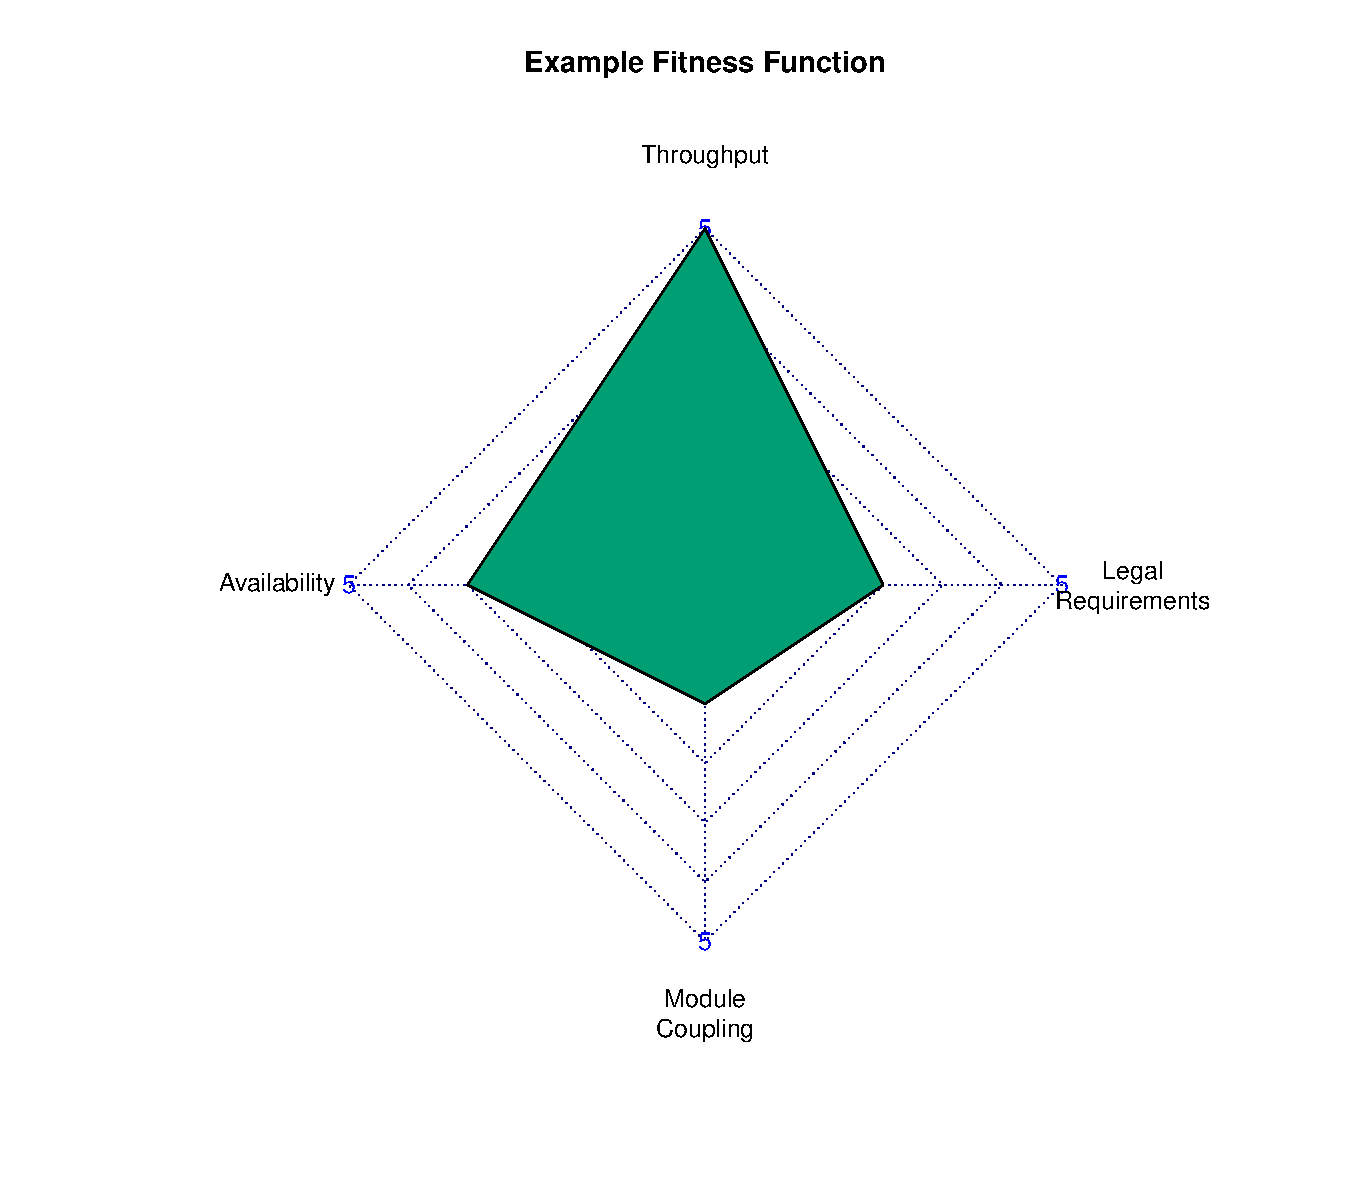
\includegraphics[width=\textwidth]{gfx/fitness-function-example}
        }
        \label{figure:fundamentals:evolutionary:fitness}
\end{figure}

\section{Controlled Experiments}
\label{sec:fundamentals:experiments}

The earliest documented controlled experiment dates back to the 1700's.
The crew of a British ship suffered from scurvy, a common suffering that sailors tend to experience when exposed to a limited diet like on sea ships during that time.
As the ship was charging citrus fruits, the captain of the ship decided to do an experiment: 50\% of his sailors, the \emph{treatment} group, had limes added to their diet.
The other half of the crew did not eat any citrus fruits; these were the \emph{control} group.
Although the reasons were not known during that moment, the experiment was a success: The treatment group got better, and eventually all sailors had citrus fruits added to their diet~\cite{rossi2003evaluation,marks2000progress}.

This anecdote is an example for one type of controlled experiment, the A/B test.
In such an A/B test, \emph{experimental units} are randomly assigned to either the control or the treatment group, which results in the group seeing the respective variant of the tested feature.
When testing a web application, the experimental unit typically is the end user.
While the treatment group is treated with the new version of the system that is being tested, the control group experiences the same system as before, without the modification.
If all users participate in the experiment, each group contains 50\% of the user base.
The results of the control group can be used in order to validate wether the treatment had any statistically significant effect~\cite{Kohavi2009}.

When executing controlled experiments, an important factor is the choice of metric that is used for comparing results.
\citet{Kohavi2013a} stress the importance of defining an \ac{OEC} which distills important metrics such as revenue or customer satisfaction in one single metric.
Having a fitting \ac{OEC} eliminates the need to carefully balance out the other metrics, as they are represented by the \ac{OEC}.
\citeauthor{Kohavi2013a} give an example where market share is a bad \ac{OEC} for a search engine, as worsening the search algorithm would increase the amount of search queries in the short term and thus increase market share; in the long run, users would use an alternative product and thus this \ac{OEC} would drop again.
Sessions per user would be a much better \ac{OEC} in this example according to \citeauthor{Kohavi2013a}.

Some additional details regarding statistical tests are of importance when A/B tests are executed in a production environment~\cite{Kohavi2009}.
These details all relate to the sample size of the experiment in some way, which is the amount of experimental units -- e.g. users -- that participate in the experiment.
The desired sample size of the finished experiment can be computed based on a variety of factors, including the desired difference in the \ac{OEC} that should be detectable and the acceptable standard error~\cite{mason2003statistical}.
The specifics of these computations are not relevant for the understanding of this thesis.

\section{Event Sourcing}
\label{sec:fundamentals:event}

%abstract: what is event sourcing
The core premise of event sourcing~\cite{WEB:Fowler:2005} is that all changes to the application state are stored as immutable events, in the order in which they occur.
In aggregation, these events represent the whole application state.

An event is a description of something that has happened in the past, such as an update of a customer's address.
In order to make this more clear, events are named as verbs in the past tense, e.g. \texttt{AddressChangedEvent}.
Event sourcing organizes these events in so-called streams.
Streams are append-only data structures, which has the benefit that a stream cannot only answer \emph{what} the current state is, but also \emph{how} the state was reached.

Inherent to event sourcing is the lack of an explicit schema, like in NoSQL databases~\cite{fowler2013schemaless}.
Instead, the schema is represented implicitly within the application itself.
This enables more flexibility, as any type of data can be saved without defining a schema first.
However, it also comes with some drawbacks, especially when this implicit schema changes~\cite{Overeem2017}.

%, contrary to classical relational databases,
\citet{Overeem2017} and \citet{Erb2016} have done some research on event sourcing and \citet{evans2004domain} grazes the topic in his book.
Apart from these few examples, literature in form of books or scientific papers regarding event sourcing is rather rare.
Several extensive blog posts by \citet{WEB:Fowler:2005} and \citet{young2010whyeventsourcing} explain the concepts and methods in great extent though.

\subsection{Features}

% what can you do with event sourcing: aggregation, rollback
When all changes to the application state are introduced via event objects, various capabilities arise which are not possible if only the application state is stored.
As \citet{WEB:Fowler:2005} describes, these are Complete Rebuild, Temporal Query, and Event Replay.

Complete rebuild means that the application state can be discarded and then rebuilt by querying all events that occurred since the beginning.
This is possible because no event in an event store is ever deleted.
Instead of doing a complete rebuild up to the present application state, the rebuild can also be done to a given date somewhere in the past.
By doing so, the application state at the given point in time is re-created, which is called a temporal query.
In another variant of the complete rebuild, called event replay, it is also possible to change a certain past event and then replay all subsequent events.
This yields a variant of the current application state reflecting the consequences introduced by the modified event.
Event replay can be done just for testing purposes, for correcting a wrong event or for fixing errors caused by events occurring in the wrong order.

If the events are designed accordingly, it is also possible to undo a given event by creating its reverse version.
This is easy if the event encodes the difference between the occurring event and the application state at that point, for example for events that add or subtract a numeral value.
Reversing of events is not that straightforward if this difference approach is not used -- the events should include the previous and updated value in that case, but this is not ideal in every case.
It is important to note that event reversability can also be achieved by reverting to a given snapshot of the application state and then replaying all events \emph{except} the event that shall be undone.

A well known example for a system which makes use of event sourcing techniques is the version control system Git\footnote{\url{http://git-scm.com/}}.
It does complete rebuilds when a project is checked out for the first time and uses temporal queries for introducing changes when switching to an existing branch.

% what can you NOT do / disadvantages
Aside from its advantages, event sourcing is not an ideal storage solution for all use cases.
First of all, event sourcing introduces a level of indirection to the application, which makes the system architecture more complicated.
Additionally, as this is an altogether different concept than storing the state directly in a database, it is thus hard to grasp and thoroughly understand for most developers.

Event sourcing uses the \acf{CQRS} pattern for separating read and write models.
The rationale behind this pattern is that the more complex a data model becomes, the more implicit representations for it exist~\cite{WEB:Fowler:2011}.
When writing to the model, additional validation logic could be executed, while multiple records may be summarized into a single one when they are read.
As this can become confusing very quickly, \ac{CQRS} strictly separates the read model from the write model.
Requests that read from the model in \ac{CQRS} are called queries, requests that write to the model are called commands.

% What about code changes?

% how some of these disadvantages can be worked around (short)
As events are immutable, event sourcing does not have a delete operation, because immutability prohibits deletion.
It is however possible to create explicit removal events -- for example a \texttt{CustomerRemoved} event for deleting a customer -- which in the end results in an application state where the item in question is not present anymore.

\subsection{Event Store: Subscriptions}

The reference implementation for a data store using event sourcing is the Event Store\footnote{\url{https://eventstore.org/}}.
It adds some features on top of the already explained event sourcing mechanics, one of which are subscriptions.
Subscriptions allow clients to be notified when new events are written to a stream.
There are three types of subscriptions:

\begin{description}
\item[Volatile Subscription]
The time at which the subscription is enabled is considered as its starting point.
All events that are written \emph{after} the starting point are considered by the subscription, prior events are ignored.
\item[Catch-Up Subscription]
This subscriptions allows the starting point to be supplied as a parameter by the client, e.g. in form of an event number.
Events that were written after the given starting point are served immediately to the client.
For all subsequently written events, the catch-up subscription behaves just as the volatile subscription.
\item[Persistent Subscription] 
This is a special kind of catch-up subscription.
The persistent subscription stores the subscription state on the server side and supports the \emph{competing consumers} messaging pattern~\cite{WEB:Microsoft-Competing-Consumers}.
This pattern supports multiple consumers which asynchronously and independently handle messages generated by the server.
In this pattern, it is not relevant which of the services handle a specific message, and every message is guaranteed to be delivered \emph{at least once}.
Therefore, it is possible to set up multiple worker services for feeding event store data into a consuming service and thus enable horizontal scalability.
\end{description}

\section{Empirical Validity}
\label{sec:fundamentals:evaluation}

When doing empirical research in the field of software engineering, it is important that the conclusions drawn from the results are in fact \emph{valid} in the eyes of the reader.
\citet{Easterbrook2008} list four factors for validity of empirical work: Construct validity, internal validity, external validity, and reliability.

Construct validity revolves around the correct interpretation and application of existing theoretical concepts of the problem domain.
Problems with construct validity occur if these concepts are not applied correctly and consistently.
For example, if the researcher doing an A/B test chooses MAC addresses as the experimental unit, construct validity is at risk because the same user can access the software on different devices with different MAC addresses.

Internal validity focuses on drawing the correct conclusions from the present results.
If the data is not interpreted correctly, internal validity is at risk.

External validity, on the other hand, focuses on the generality of the results.
If the research is conducted with a very homogenous subject group -- e.g. exclusively male test subjects -- external validity is at risk because the results would probably be different if the same research was done with a more diverse group of test subjects.

The last factor for validity of empirical work is reliability.
Reliability can be at risk if the researcher has a bias of some sort.
\citeauthor{Easterbrook2008} explicitly mention that it can be problematic if the researcher has personal stakes in the software under test.

\section{Docker}
\label{sec:fundamentals:docker}

Docker\footnote{\url{https://www.docker.com/}} is a container platform that allows for lightweight and flexible virtualization of services and applications.
The central concept of Docker are its containers, which package application code as well as dependent libraries, binaries, and settings.
It is important to note that a Docker container does not contain a host operating system -- a main difference between a container and a \ac{VM}.
This makes containers more lightweight than \ac{VM}s, resulting in a usually smaller footprint in terms of CPU usage, main memory, and storage.
A container is executed by the Docker engine, which is amongst others available for Linux, Windows and MacOS.

Docker containers are defined by a \emph{Dockerfile}, which hosts a set of instructions that tell the Docker engine how to build the image which in the end is instantiated in a container.
\Cref{code:fundamentals:docker:dockerfile} shows an exemplary Dockerfile.
Each instruction of the Dockerfile creates another filesystem layer, which in combination produce the final image.
In the printed example, the Dockerfile states that the base image shall be the \texttt{nginx} image\footnote{\url{https://www.nginx.com/}} with version \texttt{1.13}.
This instruction creates the first image layer.
The \texttt{COPY} instruction copies the contents of the folder where the Dockerfile resides into the stated destination in the target filesystem, such that the copied files can be served by the NGINX instance.
This creates the second image layer.
It is very important to note that the Docker engine saves image layers as diffs, meaning that a layer is described by its  difference with the layer below.
This results in faster rebuild times for containers: When the \texttt{COPY} instruction in the example Dockerfile is changed, only the second image layer has to be rebuilt.
%This suffices to bootstrap the containers itself, but in most cases additional configuration files are loaded into the container via volumes.

\lstinputlisting[label={code:fundamentals:docker:dockerfile},caption={Example Dockerfile}]{sourcecode/Dockerfile.txt}

Containers can be created and run via the Docker \ac{CLI}.
For example, the custom NGINX image previously described in \cref{code:fundamentals:docker:dockerfile} would first be containerized and then executed via the instructions given in \cref{code:fundamentals:docker:cli}.
The \texttt{-p} option specifies that the container's port 80 shall be exposed as port 8000 on the host operating system.

\lstinputlisting[label={code:fundamentals:docker:cli},caption={Commands for building and running the NGINX example container via the Docker CLI},language=bash]{sourcecode/docker-cli.sh}

However, building and running images and containers via the Docker \ac{CLI} becomes tedious when a combination of multiple containers has to be managed.
\emph{Docker Compose} facilitates container composition by storing these build and run definitions in a single configuration file, using the data serialization language \ac{YAML}.
\Cref{code:fundamentals:docker:compose-yml} shows an exemplary \texttt{docker-compose.yml} file, which specifies that  the previously shown Dockerfile shall be used for building the image as a service called \texttt{server}, and that again port 8000 shall be exposed.
The image is then built, and the container subsequently run, via two commands as shown in \cref{code:fundamentals:docker:compose-run}.
While the approach using the Docker CLI may seem more concise in this limited example, Compose's advantages when combining multiple interconnected services become apparent when doing more complex container composition (cf. \cref{sec:implementation:orchestration}).

\lstinputlisting[label={code:fundamentals:docker:compose-yml},caption={Example docker-compose.yml}]{sourcecode/docker-compose-example.yml}
\lstinputlisting[label={code:fundamentals:docker:compose-run},caption={Commands for building and running the NGINX example container via Compose},language=bash]{sourcecode/run-via-compose.sh}

The container architecture of Docker solves two challenges when creating distributed systems: application independence and bridging the gap between development and operations.
Application independence is achieved by running every application in its own container which can only interact with other containers via explicitly defined interfaces (e.g. HTTP).
Docker facilitates bridging the gap between the developers and operations teams, as the environment that the application is executed in -- the Docker container -- does not change between the development and production stages.
This makes Docker a popular technology for implementing DevOps.

Instead of Docker, a few alternative technologies could have been chosen as the virtualization solution.
These alternatives include services such as Vagrant, Kubernetes and Apache Mesos, some of which make use of Docker internally.
Docker was favored over the alternatives because of its maturity, good documentation, and previous personal experience with it -- making this a partly subjective decision.
It would also be possible to run the passive user feedback system natively on a server or multiple servers, but this would have introduced unnecessary complications.